\documentclass[12pt]{article}

% Packages for enhanced typesetting and functionality
\usepackage{amsmath, amssymb, amsthm}      % Math symbols and environments
\usepackage{graphicx}                      % For including images
\usepackage{fancyhdr}                      % For header and footer customisation
\usepackage{geometry}                      % For margin customisation
\usepackage[colorlinks=true, linkcolor=blue, urlcolor=blue, citecolor=blue]{hyperref} % Clickable links
\usepackage{xcolor}                        % For coloured text
\usepackage{tikz}                          % For drawing diagrams and flowcharts
\usepackage{algorithm}                     % For algorithms
\usepackage[noend]{algpseudocode}          % For algorithm pseudocode

% Page layout settings
\geometry{margin=1in}
\setlength{\parindent}{0pt}
\setlength{\parskip}{1ex}

% Header and footer
\pagestyle{fancy}
\fancyhf{}
\setlength{\headheight}{15pt}
\fancyhead[L]{Solving Air Crew Scheduling Problems}
\fancyhead[R]{Max Hart}
\fancyfoot[C]{\thepage}

\begin{document}

% Title Page
\begin{titlepage}
    \centering
    \vspace*{1cm}
    
    % University logo (adjust image file as needed)
    
\includegraphics[width=0.4\textwidth]{UoB.jpg}\par\vspace{1cm}
    
    {\LARGE\bfseries Solving Air Crew Scheduling Problems\par}
    \vspace{0.5cm}
    {\Large A Simulated Annealing and Genetic Algorithm Approach\par}
    \vspace{0.75cm}
    
    {\large Evolutionary Computation\par}
    \vspace{1.5cm}
    
    {\large\textbf{Author:} Max Hart\par}
    \vspace{0.3cm}
    {\normalsize \href{mailto:mah422@student.bham.ac.uk}{mah422@student.bham.ac.uk}\par}
    \vspace{1.5cm}
    
    {\large\textbf{Professors:} Dr Shan He and Dr Per Kristian Lehre\par}
    \vspace{1cm}
    
    {\large \today\par}
    
\end{titlepage}

\tableofcontents
\newpage

\section{Introduction}
Airline crew scheduling is widely recognised as one of the most challenging and practically significant optimisation problems in the transportation industry. Typically modelled as a Set Partitioning Problem (SPP), the task involves assigning each flight leg to a valid crew rotation—ensuring every leg is covered exactly once—while satisfying a multitude of operational constraints. Owing to the enormous combinatorial complexity inherent in real-world instances, conventional exact methods are often inadequate. This has spurred the development of advanced metaheuristic techniques that are capable of delivering high-quality, near-optimal solutions within a reasonable computational time.

The motivation for this project is threefold:
\begin{itemize}
    \item \textbf{Scalability:} To address the limitations of exact methods in handling large-scale, real-world scheduling instances.
    \item \textbf{Robustness:} To develop algorithms that reliably navigate complex search landscapes and overcome local optima.
    \item \textbf{Innovation in Constraint Handling:} To integrate state-of-the-art techniques—such as pseudo–random initialisation, heuristic improvement operators, and stochastic ranking—to effectively manage the stringent constraints of the SPP.
\end{itemize}

In pursuit of these objectives, we have implemented three distinct algorithms from scratch:
\begin{itemize}
    \item \textbf{Simulated Annealing (SA)}
    \item \textbf{Standard Binary Genetic Algorithm (BGA)}
    \item \textbf{Improved Binary Genetic Algorithm (BGA)}
\end{itemize}
The improved variant is particularly noteworthy, as it incorporates problem-specific enhancements inspired by Chu \& Beasley~\cite{ChuAndBeasley1998} and Runarsson and Yao~\cite{RunarssonYao2000}. Our ambition is not only to demonstrate the correctness and efficiency of these approaches on three OR–Library test instances (sppnw41, sppnw42, and sppnw43) over 30 independent runs, but also to conduct a detailed comparative analysis of their performance, convergence behaviour, and constraint-handling strategies.

Through this work, we aspire to contribute valuable technical insights into the application of metaheuristic techniques for solving complex, real-world scheduling problems.

\section{Algorithm Descriptions}
\label{sec:algorithms}
In this section, we provide a comprehensive overview of the three algorithms developed for solving the SPP. For each algorithm, we begin with a brief introduction that outlines its underlying principles and technical merits, followed by the corresponding pseudocode. Detailed flowcharts, which visually encapsulate the step-by-step processes, are presented on subsequent pages. Our aim is to clearly elucidate the operational mechanics and innovative aspects of each method.

\subsection{Simulated Annealing (SA)}
Simulated Annealing is a local search technique that iteratively improves a candidate solution by exploring its neighbourhood. It uses a temperature parameter to probabilistically accept inferior solutions, thereby enabling the algorithm to escape local optima. This simple yet effective approach balances exploration and exploitation through gradual cooling.

\subsubsection{Pseudocode}
The pseudocode below outlines the Simulated Annealing algorithm applied to the Set Partitioning Problem. It details the initialization of a random solution, the iterative process of generating and evaluating a neighbor via bit-flipping, the acceptance decision using both direct improvement and the Metropolis criterion, and finally, the gradual cooling of the system.

\begin{algorithm}[htbp]
  \caption{SimulatedAnnealing(\(T\), \(\alpha\), maxIter, penaltyFactor)}
  \begin{algorithmic}[1]
    \State \(x \gets \text{RandomSolution}()\) \Comment{Generate a random binary solution}
    \State \(F(x) \gets \text{PenaltyFitness}(x,\,\text{penaltyFactor})\)
    \State \(x_{\text{best}} \gets x,\; F_{\text{best}} \gets F(x)\)
    \For{\(iter = 1\) to maxIter}
      \State \(x' \gets \text{FlipOneRandomBit}(x)\) \Comment{Generate a neighbor solution by flipping one bit}
      \State \(F(x') \gets \text{PenaltyFitness}(x',\,\text{penaltyFactor})\)
      \If{\(F(x') < F(x)\)}
        \State \(x \gets x'\) \Comment{Accept the neighbor if it is better}
      \Else
        \State \(\Delta \gets F(x') - F(x)\)
        \If{\(\text{rand}() < e^{-\Delta/T}\)}
          \State \(x \gets x'\) \Comment{Accept with probability \(e^{-\Delta/T}\) (Metropolis criterion)}
        \EndIf
      \EndIf
      \If{\(F(x) < F_{\text{best}}\)}
        \State \(x_{\text{best}} \gets x,\; F_{\text{best}} \gets F(x)\) \Comment{Update best solution if improved}
      \EndIf
      \State \(T \gets \alpha \, T\) \Comment{Cool down the temperature}
    \EndFor
    \State \Return \((x_{\text{best}}, F_{\text{best}})\)
  \end{algorithmic}
  \end{algorithm}

\subsubsection{Flowchart}
The accompanying flowchart visually represents the step-by-step flow of the Simulated Annealing algorithm. It clearly illustrates each phase—from initial solution generation, neighbor evaluation, and acceptance decisions to the temperature update—providing an intuitive overview of the algorithm’s operational dynamics.

\begin{figure}[htbp]
  \centering
  % Adjust the width as needed, e.g., 0.9\textwidth fills most of the page width
  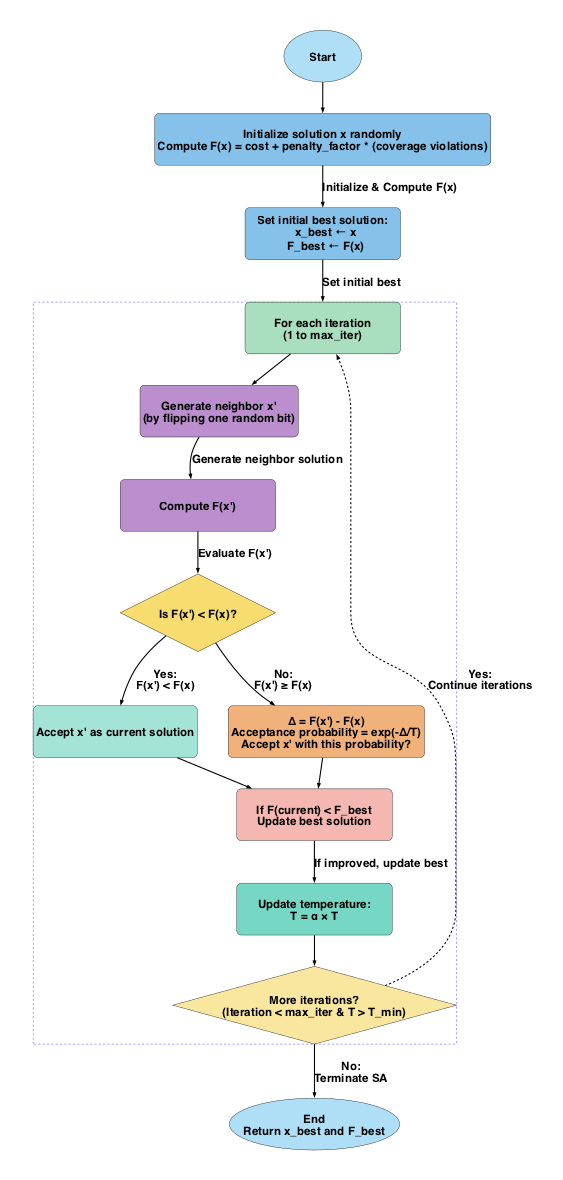
\includegraphics[width=0.60\textwidth]{simulated_annealing_flowchart.png}
  \caption{Flowchart of the Simulated Annealing Algorithm for the Set Partitioning Problem.}
  \label{fig:flowchart1}
\end{figure}

\newpage

\subsection{Standard Binary Genetic Algorithm (BGA)}
The Standard Binary Genetic Algorithm is a population-based technique that evolves a set of candidate solutions using selection, crossover, and mutation operators. It utilises tournament selection to choose parents, applies one-point crossover to combine their genetic material, and uses bit-flip mutation to introduce variability. A penalty function is employed to combine the cost of a solution with constraint violations, ensuring that feasibility is encouraged over generations. This method is well-suited for problems with discrete binary representations and offers robustness through its stochastic operations.

\subsubsection{Pseudocode}
\begin{algorithm}[htbp]
\caption{StandardBGA(popSize, cxRate, mutRate, maxGens, penaltyFactor, tournamentK)}
\begin{algorithmic}[1]
  \State \(P \gets \text{RandomPopulation}(popSize)\)
  \State \(\text{EvaluateFitness}(P,\,\text{penaltyFactor})\)
  \For{\(g = 1\) to maxGens}
    \State \(Q \gets \emptyset\)
    \While{\(|Q| < \text{popSize}\)}
      \State \(p_1 \gets \text{TournamentSelect}(P,\, tournamentK)\)
      \State \(p_2 \gets \text{TournamentSelect}(P,\, tournamentK)\)
      \If{\(\text{rand}() < cxRate\)}
        \State \((c_1, c_2) \gets \text{OnePointCrossover}(p_1, p_2)\)
      \Else
        \State \(c_1 \gets p_1,\; c_2 \gets p_2\)
      \EndIf
      \State \(\text{Mutate}(c_1,\, mutRate)\)
      \State \(\text{Mutate}(c_2,\, mutRate)\)
      \State \(\text{EvaluateFitness}(\{c_1, c_2\},\, \text{penaltyFactor})\)
      \State \(Q \gets Q \cup \{c_1, c_2\}\)
    \EndWhile
    \State \(P \gets Q\)
  \EndFor
  \State \Return \(\text{BestSolution}(P)\)
\end{algorithmic}
\end{algorithm}

\subsubsection{Flowchart}
\begin{figure}[htbp]
  \centering
  % Adjust the width as needed, e.g., 0.9\textwidth fills most of the page width
  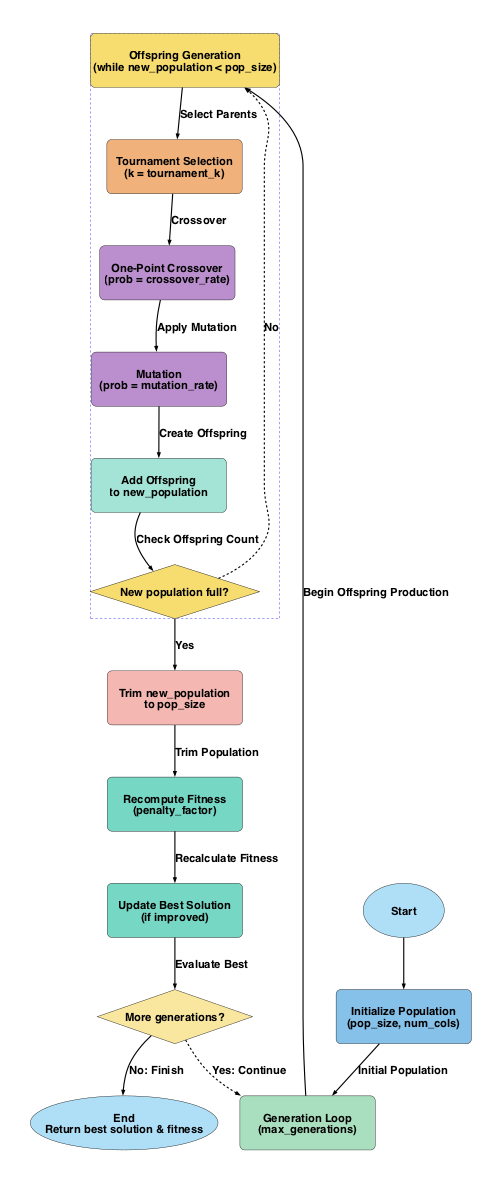
\includegraphics[width=0.55\textwidth]{standard_bga_flowchart.png}
  \caption{Flowchart of the Standard Binary Genetic Algorithm for the Set Partitioning Problem.}
  \label{fig:flowchart2}
\end{figure}

\newpage

\subsection{Improved Binary Genetic Algorithm (BGA)}
The Improved Binary Genetic Algorithm extends the standard BGA by integrating several problem-specific enhancements. It begins with a pseudo–random initialisation that aims to reduce over–coverage in the initial population. The algorithm then incorporates a stochastic ranking procedure that probabilistically balances cost and constraint violation, allowing for a more flexible handling of infeasible solutions. Adaptive mutation is employed to reintroduce promising genetic material, and a DROP/ADD heuristic improvement operator repairs infeasible solutions. These enhancements, inspired by Chu \& Beasley~\cite{ChuAndBeasley1998} and Runarsson \& Yao~\cite{RunarssonYao2000}, make the Improved BGA particularly robust for the SPP. Overall, this algorithm offers a more sophisticated search mechanism by blending global search operators with domain-specific repairs.

\subsubsection{Pseudocode}
\begin{algorithm}[htbp]
\caption{ImprovedBGA(popSize, maxGens, \(p_{\mathrm{stoch}}\), ...)}
\begin{algorithmic}[1]
  \State \(P \gets \text{PseudoRandomInit}(popSize)\)
  \State \(\text{EvaluateCostUnfitness}(P)\)
  \For{\(g = 1\) to maxGens}
    \State \(\text{StochasticRankSort}(P, p_{\mathrm{stoch}})\)
    \State \(O \gets \emptyset\)
    \While{\(|O| < popSize\)}
      \State \((p_1, p_2) \gets \text{SelectParents}(P)\)
      \State \((c_1, c_2) \gets \text{UniformCrossover}(p_1, p_2)\)
      \State \(\text{AdaptiveMutation}(c_1, P)\)
      \State \(\text{AdaptiveMutation}(c_2, P)\)
      \State \(\text{HeuristicImprove}(c_1)\)
      \State \(\text{HeuristicImprove}(c_2)\)
      \State \(\text{EvaluateCostUnfitness}(\{c_1, c_2\})\)
      \State \(O \gets O \cup \{c_1, c_2\}\)
    \EndWhile
    \State \(C \gets P \cup O\)
    \State \(\text{StochasticRankSort}(C, p_{\mathrm{stoch}})\)
    \State \(P \gets \text{Top}(C, popSize)\)
  \EndFor
  \State \Return \(\text{BestFeasible}(P)\)
\end{algorithmic}
\end{algorithm}

\subsubsection{Flowchart}
\begin{figure}[htbp]
  \centering
  % Adjust the width as needed, e.g., 0.9\textwidth fills most of the page width
  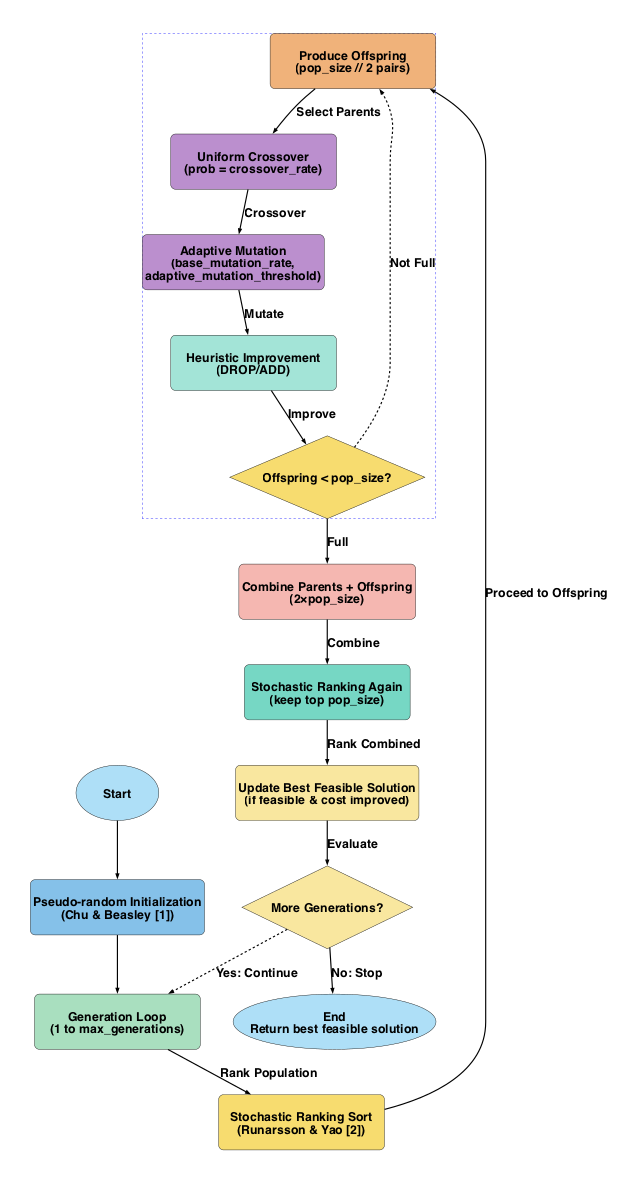
\includegraphics[width=0.70\textwidth]{improved_bga_flowchart.png}
  \caption{Flowchart of the Improved Binary Genetic Algorithm for the Set Partitioning Problem.}
  \label{fig:flowchart3}
\end{figure}

\newpage

\section{Benchmark Results}
\label{sec:results}


\section{Discussion and Comparison}
\label{sec:discussion}

\newpage

\section{Ranking Replacement vs. Stochastic Ranking}
\label{sec:ranking}
Both methods aim to balance cost and constraint satisfaction in the SPP, yet they differ in approach. The \textbf{Ranking Replacement} method (Chu \& Beasley, 1998) partitions the population deterministically into four subgroups based on fitness (cost) and unfitness (constraint violation). A new solution replaces an individual from the first non-empty subgroup (starting with those worst in both criteria), thereby steadily improving the overall population. This approach offers a clear structure but can be rigid as the balance between cost and constraint violation may evolve during the search.

In contrast, the \textbf{Stochastic Ranking} method (Runarsson \& Yao, 2000) uses a bubble-sort-like procedure where adjacent solutions are compared probabilistically—if at least one solution is infeasible, they are compared by cost with a set probability \(P\) (typically less than 0.5) and by unfitness otherwise. This allows for a more adaptive balance, enabling the search to explore infeasible regions as bridges between isolated feasible areas without rigid subgroup thresholds.

In summary, while both methods share the goal of guiding the search toward feasible, high-quality solutions, Ranking Replacement enforces a strict hierarchical structure, whereas Stochastic Ranking offers a flexible, adaptive mechanism that reduces the need for extensive parameter tuning.
\section{Conclusion}
This report has presented three advanced algorithms for solving airline crew scheduling problems: Simulated Annealing, a Standard Binary Genetic Algorithm, and an Improved Binary Genetic Algorithm incorporating problem-specific enhancements. Detailed, moderately sized flowcharts and refined pseudocode have been provided to elucidate each method's internal workings. Benchmark results and an in-depth discussion will be appended once experiments are complete. Furthermore, a comparative discussion on constraint-handling—contrasting ranking replacement and stochastic ranking—has been included, underscoring the adaptive advantages of the latter.

\newpage

\begin{thebibliography}{9}
\bibitem{ChuAndBeasley1998}
  P.~C. Chu and J.~E. Beasley, 
  \emph{Constraint Handling in Genetic Algorithms: The Set Partitioning Problem},
  Journal of Heuristics, 11:323--357, 1998.

\bibitem{RunarssonYao2000}
  T.~P. Runarsson and X. Yao, 
  \emph{Stochastic Ranking for Constrained Evolutionary Optimisation},
  IEEE Transactions on Evolutionary Computation, 4(3):284--294, 2000.
\end{thebibliography}

\end{document}